

\section{Inhalt SE2}

\section*{1. Objektorientierte Analyse}

\subsection*{Lernziele}
\begin{itemize}
    \item verstehen, wie und wozu Modelle in Analyse und Entwurf verwendet werden
    \item wissen, wie Objekte und Klassen zur Analyse von Anforderungen der Software verwendet werden
    \item Klassendiagramme der Analyse auf systematische Art und Weise erstellen können
    \item Nutzen von Mustern beurteilen können
    \item den Aufbau von Mustern verstehen
    \item die wichtigsten Analysemuster kennen und verwenden können
    \item Konzepte zum systematischen Entwurf und zur ergonomischen Gestaltung von Benutzeroberflächen kennen
\end{itemize}

\subsection*{Zusammenfassung}
\begin{itemize}
    \item in der \textbf{Analyse} werden \textbf{Modelle} genutzt, um Anforderungen zu verstehen und Lösungen aus fachlicher Sicht zu entwickeln
    \item hierzu werden Modelle des Umfelds und der Lösung auf formalisierte Art erstellt
    \item diese dienen den Modellen des \textbf{Entwurfs}
    \item Modelle bestehen aus \textbf{statischen} und \textbf{dynamischen} Modellteilen, wobei statische Modellteile die Teile und ihre Beziehungen untereinander modellieren, und dynamische das Zusammenspiel der Teile beschreiben
    \item In der OO-Analyse wird statische Modellierung mit \textbf{Klassendiagrammen} realisiert.
    \item[] Dynamische Modelle, die Zustände und Übergänge von Zuständen beschreiben, werden mittels \textbf{Zustandsdiagrammen} modelliert.
    \item[] Beschreiben dynamische Modelle Abläufe von Aktivitäten, nutzt man \textbf{Aktivitätsdiagramme}.
    \item Bei der Analyse kommen außerdem Analysemuster zum Einsatz: Muster beschreiben Lösungskizzen verallgemeinerter Probleme
    \item[] Sie helfen, indem sie \textbf{bewährte Lösungen} beschreiben und ein \textbf{Kommunikationsmittel} darstellen
    \item Die wichtigsten Analysemuster sind \textbf{Exemplartyp}, \textbf{Wechselnde Rollen} und \textbf{Allgemeine Hierarchie}.
    \item Die Gestaltung der Benutzeroberfläche ist Bestandteil der Analyse, wobei logische Struktur, die Informationsarchitektur und die physische Gestalt entworfen werden.
    \item[] Ergonomie und Barrierefreiheit sind wichtige Punkte, die dabei beachtet werden müssen.
\end{itemize}

\section*{2. Architektur}

\subsection*{Lernziele}
\begin{itemize}
    \item verstehen, was Architektur ist und welchen Einflüssen sie unterliegt
    \item die wichtigsten Architekturmuster kennen und einordnen können
\end{itemize}

\subsection*{Zusammenfassung}

\begin{itemize}
    \item Der grundlegende Aufbau einer Software wird über die \textbf{Softwarearchitektur} beschrieben.
    \item Die Architektur sollte aufgrund ihrer grundsätzlichen Bedeutung von Anfang an berücksichtigt werden.
    \item Grundlage für eine Architektur sind Anforderungen und Randbedingungen, wobei \textbf{nicht-funktionale Anforderungen} und \textbf{Randbedingungen} entscheidenden Einfluss haben.
    \item Hilfsmittel für eine Softwarearchitektur sind \textbf{Taktiken}, \textbf{Muster} (bspw. Client-Server, Schichtenbildung) und \textbf{Referenzarchitekturen}.
    \item Die Dokumentation von Architekturen erfolgt in \textbf{Sichten}.
\end{itemize}

\section*{3. Objektorientierter Entwurf}

\subsection*{Lernziele}
\begin{itemize}
    \item verstehen, wie und wozu Modelle im Entwurf verwendet werden
    \item Zusammenhang zwischen Modellen der Analyse und des Entwurfs verstehen
    \item Klassendiagramme des Entwurfs auf systematische Art und Weise erstellen können
    \item bei der Erstellung von Entwürfen Entwurfsmuster verwenden können
    \item die Qualität von Entwürfen beurteilen und systematisch verbessern können
\end{itemize}

\subsection*{Zusammenfassung}

\begin{itemize}
    \item im \textbf{Entwurf} werden Klassen und Dateien eines zu entwerfenden Systems \textbf{geplant}
    \item dabei beruht der Entwurf auf den \textbf{Anforderungen}, den \textbf{Ergebnissen der Analyse} und der \textbf{Architektur}
    \item die Klassen des Entwurfs entsprechen den Klassen der verwendeten objektorientierten Sprache
    \item die \textbf{Struktur der Klassen} wird mit \textbf{UML-Klassendiagrammen} definiert
    \item \textbf{Abläufe} und das \textbf{Zusammenspiel} von Klassen wird mit \textbf{UML-Sequenzdiagrammen} modelliert
    \item der Entwurf sollte sinnvollerweise \textbf{schrittweise} (\texit{iterativ}) entwickelt werden
    \item hierbei helfen grundlegende Prinzipien wie ``\textit{Reise mit leichtem Gepäck}``
    \item Entwurfsmuster wie \textbf{Beobachter}, \textbf{MVC} und \textbf{Fassade} sind wichtige Hilfsmittel beim Entwurf
    \item anhand von \textbf{Prinzipien guten Entwurfs} kann die \textbf{Qualität eines Entwurfs} beurteilt werden
    \item das wichtigste Prinzip hierbei ist die Aufteilung der Gesamtaufgabe in \textbf{kleine Teile}, wobei die Teile lose untereinander gekoppelt sein sollen, was durch eine \textbf{hohe Kohäsion} (\textit{Zusammenhalt}) sowie \textbf{Vermeidung starker Kopplung} (Globale Variablen, lange formale Parameterlisten in den Methoden-Signaturen usw.) erreicht werden kann, außerdem durch die Beachtung guten Entwurfs wie Vermeidung zirkulärer Abhängigkeiten
    \item die Qualität eines Entwurfs bleibt gut, indem der Code durch \textbf{Refactorings} stetig verbessert wird
\end{itemize}

\clearpage

\section{Analyse- und Entwurfsphase}

\begin{tcolorbox}[title=Analysephase]
    Nach der \textbf{Anforderungsphase} wird in der \textbf{Analysephase} ein formales Modell sowohl des Problems in seinem Umfeld als auch der Lösung erstellt.\\
    Die Analyse beschreibt fachliche Zusammenhänge, keine technische.
\end{tcolorbox}

\begin{tcolorbox}[title=Entwurfsphase]

In der \textbf{Entwurfsphase} wird die \textbf{Architektur} der Anwendung bestimmt, unter Berücksichtung technischer Randbedingungen, die im Rahmen nicht-funktionaler Anforderungen in der Anforderungsphase gesammelt wurden und vom Kunden stammen.\\
Die Architektur schließt u.a. ein:

\begin{itemize}
    \item Programmiersprache
    \item Frameworks
    \item Einsatz von Datenbanken
    \item \ldots
\end{itemize}

\noindent
Meist bleiben im Anschluss technische Fragen offen, die im weiteren Verlauf dieser Phase beantwortet werden, z.B.:

\begin{itemize}
    \item Welche \textbf{Klassen} aus der \textbf{Analyse} können übernommen werden?
    \item Wie werden Klassen in einem relationalen Datenbank-Schema gespeichert?
    \item Welche Steuerungsklassen müssen für die GUI implementiert werden?
\end{itemize}
\end{tcolorbox}

\clearpage

\section{Modell}



\vspace{2mm}
\begin{tcolorbox}[title=Arbeitsdefinition ``Modell``]
    Ein \textbf{Modell} ist ein Produkt des \textbf{Modellierungsvorgangs}.\\

    \noindent
    Es beschreibt tatsächliche oder gedachte Gegenstände oder Konzepte und deren Beziehungen.\\

    \noindent
    Ein Modell erfasst diese Konzepte nicht vollständig, sondern \textbf{abstrakt}, also verkürzt und vereinfacht (vgl. \cite[2]{Wed09b}).
\end{tcolorbox}
\vspace{2mm}
\clearpage

\section{Liskovsches Substitutionsprinzip / Polymorphie}

\begin{tcolorbox}[title=Liskovsches Substitutionsprinzip / Polymorphie]
Eine Bedeutung der Vererbungsbeziehung ist, dass eine Instanz einer Klasse genauso verwendet werden kann wie eine Instanz seiner übergeordneten Klasse.\\
Allgemein fasst man dies unter \textbf{Polymorphie} zusammen.\\
Als Konsequenz folgt, dass immer dann, wenn ein bestimmter Typ gefordert wird, auch sein Untertyp erlaubt ist (vgl.~\cite[466]{Ull23}), was der Kern des \textit{Liskovschen Substitutionsprinzips}\footnote{
    ``Wikipedia - Liskov substitution principle``: \url{https://en.wikipedia.org/wiki/Liskov_substitution_principle}, abgerufen 11.04.2024
}\footnote{
    s.a. ``Wikipedia - Covariance and Contravariance``: \url{https://en.wikipedia.org/wiki/Covariance_and_contravariance_(computer_science)}, , abgerufen 11.04.2024
} ist.\\

\noindent
Für die Beziehung zwischen einer abgeleiteten Klasse und ihrer Superklasse muss gelten \textbf{kann verwendet werden als} und \textbf{ist ein}.
\end{tcolorbox}

\clearpage

\section{Domänenmodell}

\begin{tcolorbox}[title=Domänenmodell]
Der Begriff \textbf{Domäne} bezeichnet das fachliche Umfeld der Aufgabe.\\

\noindent
Das \textbf{Domänenmodell} ist das \textit{statische Modell} der Domäne und basiert auf den Anforderungen und den in der \textbf{Anforderungsphase} gesammelten Informationen.\\

\noindent
In der \textbf{Analysephase} wird das Domänenmodell in Form von Klassendiagrammen erstellt.
Es beschreibt damit


\begin{itemize}
    \item welche Klassen es in einer Domäne gibt
    \item wie diese Klassen ausgeprägt sind
    \item welche Beziehungen sie untereinander haben
\end{itemize}
\end{tcolorbox}
\clearpage

\section{Analysemuster}

\begin{tcolorbox}[title=Analysemuster]
    Im Software Engineering versteht man unter dem Begriff \textit{Muster} (\textit{Pattern}) \textbf{vorgefertigte Lösungsschablonen für verallgemeinerte Probleme}.\\
    Die Beschreibung der verallgemeinerten Probleme und Lösungen auf eine \textbf{formalisierte Weise} nennt man \textbf{Muster}.\\
    Muster müssen zur Anwendung auf ein konkretes Problem \textit{konkretisiert} werden.\\
    Im Bereich des Software Engineerings gibt es Muster für \textbf{Analyse}, \textbf{Architektur}, \textbf{Entwurf}.\\

    \noindent
    \textbf{Vorteile}:
    \begin{itemize}
        \item es stehen \textbf{bewährte Standardlösungen} zur Verfügung
        \item Verwendung bereits bewährter Lösungen ist oft \textbf{schneller und besser} als selbstentwickelte neue Lösungen
        \item Muster helfen bei der \textbf{Kommunikation}
    \end{itemize}
\end{tcolorbox}

\begin{tcolorbox}[title=Beispiele]
    \begin{itemize}
        \item \textbf{Exemplartyp} (Abstraction-Occurence): Objekte einer Klasse ähneln sich untereinander und tragen gemeinsamen, gleiche Informationen oder besitzen gleiches  Verhalten, unterscheiden sich aber wesentlich
        \item \textbf{Wechselnde Rollen} (Player- Role): ein Objekt kann in unterschiedlichen Kontexten verschiedene Verantwortlichkeiten und Beziehungen haben
        \item \textbf{Allgemeine Hierarchie} (General Hierarchy, Kompositum): Objekte können hierarchisch angeordnet sein;
         jedes Objekt kann maximal einem Objekt untergeordnet sein;
         manche Objekte dieser Hierarchie können keine untergeordneten Objekte haben
    \end{itemize}
\end{tcolorbox}

\begin{figure}
    \centering
    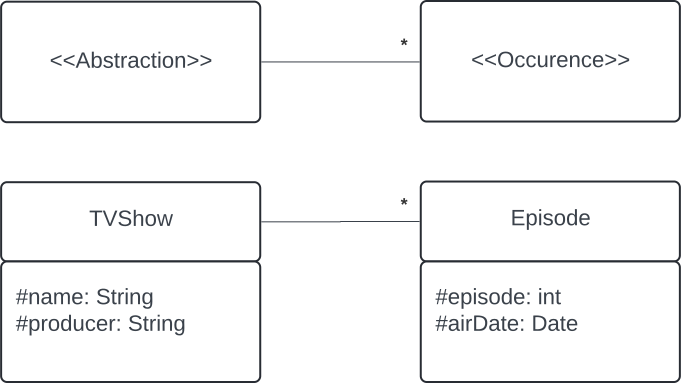
\includegraphics[scale=0.3]{part two/Objektorientierte Analyse/img/abstractionoccurence}
    \caption{Beispiel für das \textit{Abstraction-Occurence-Pattern}. (Quelle: eigene)}
    \label{fig:abstractionoccurence_cc}
\end{figure}
\begin{figure}
    \centering
    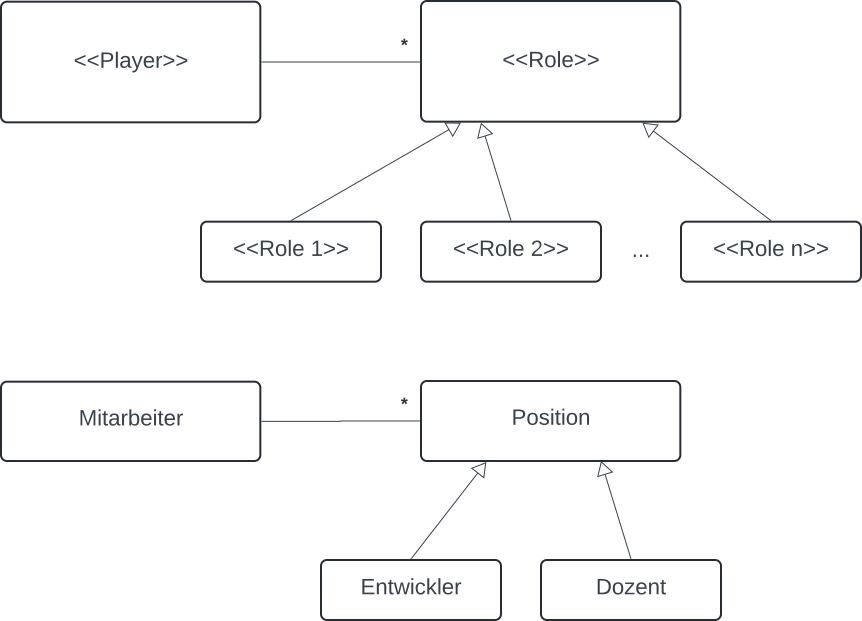
\includegraphics[scale=0.3]{part two/Objektorientierte Analyse/img/playerrole}
    \caption{Beispiel für das \textit{Player-Role-Pattern}. (Quelle: eigene)}
    \label{fig:playerrole_cc}
\end{figure}
\begin{figure}
    \centering
    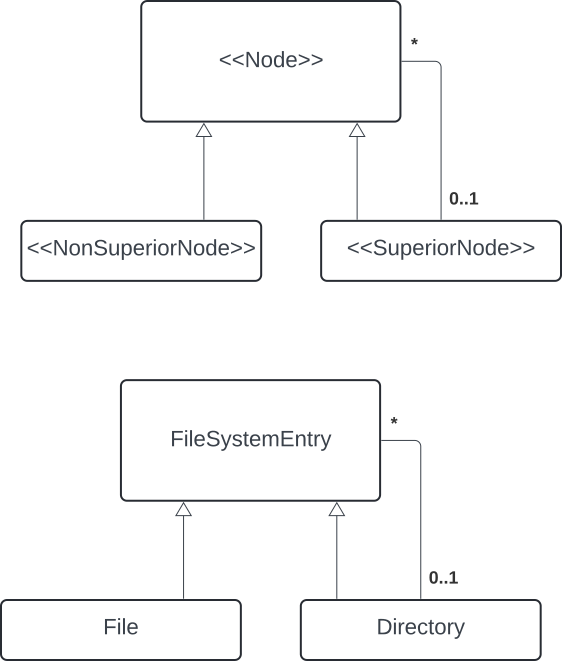
\includegraphics[scale=0.3]{part two/Objektorientierte Analyse/img/generalhierarchy}
    \caption{Beispiel für das \textit{General-Hierarchy-Pattern}. (Quelle: eigene)}
    \label{fig:generalhierarchy_cc}
\end{figure}
\clearpage

\section{Dialoggestaltung}

\begin{tcolorbox}[title=Grundsätze der Dialoggestaltung]
    Für die Gestaltung von Benutzeroberflächen sind 7 Gestaltungsgrundsätze relevant (nach \textbf{DIN EN ISO 9241}\footnote{
        s. \url{https://de.wikipedia.org/wiki/ISO_9241}, abgerufen 13.04.2024
    }):

    \begin{itemize}
        \item \textbf{Aufgabenangemessenheit}: Ein Dialog ist den Aufgaben angemessen, wenn er die Benutzer unterstützt, die Aufgaben effektiv und effizient zu erledigen.
        \item \textbf{Selbstbeschreibungsfähigkeit}: Für die Benutzer ist jederzeit offensichtlich, im welchem Dialog und an welcher Stelle im Dialog sie sich befinden, welche Handlungen unternommen werden und wie diese ausgeführt werden können.
        \item \textbf{Steuerbarkeit}: Der Benutzer ist in der Lage, den Dialogablauf zu starten und seine Richtung und Geschwindigkeit zu ändern, bis das Ziel erreicht ist (bspw. Rückgängigmachfunktion, Vor-/Zurück-Buttons \ldots).
        \item \textbf{Erwartungskonformität}: Ein Dialog ist erwartungskonform, wenn er konsistent ist und den Merkmalen des Benutzers entspricht (Kenntnisse Arbeitsgebiet, Ausbildung, Erfahrung, allgemein anerkannte Konventionen, bspw. einheitliche Verwendung von Funktionscodes und Funktionstasten in allen Dialogen).
        \item \textbf{Fehlertoleranz}: Das beabsichtigte Arbeitsergebnis wird trotz erkennbar fehlerhafter Eingaben mit keinem oder \textbf{minimalen Korrekturaufwand} seitens des Benutzers erreicht.
        \item \textbf{Individualisierbarkeit}: Das Dialogsystem erlaubt Anpassungen an Erfordernisse der Arbeitsaufgabe sowie individuelle Fähigkeiten und Vorlieben des Benutzers.
        \item \textbf{Lernförderlichkeit}: Der Benutzer wird beim Erlernen des Dialogs unterstützt und angeleitet (bspw. über ``Shortcuts`` bzw. \textit{Mnemonics}\footnote{
            s. \url{https://en.wikipedia.org/wiki/Mnemonics_(keyboard)}, abgerufen 26.04.2024
        } (vgl.~\cite[147]{Rau07f})).

    \end{itemize}
\end{tcolorbox}
\clearpage

\input{chapters/Anhang/CheatSheets/SE2/SoftwareArchitektur}
\clearpage

\section{Objektorientierter Entwurf}


\begin{tcolorbox}[title=Objektorientierter Entwurf]
    \noindent
    Der \textbf{objektorientierte Entwurf} beinhaltet
    \begin{itemize}
        \item das Erstellen von Klassen samt deren Attribute und Methode
        \item das Festlegen der Assoziationen und Vererbungsbeziehungen
        \item das Beschreiben des Zusammenspiels der Instanzen
    \end{itemize}
Der Entwurf geschieht auf Grundlage der Anforderungen und der Ergebnisse der Analyse und innerhalb der gewählten Architektur.\\
Aus den Anforderungen sind für den Entwurf die \textbf{funktionalen Anforderungen} wichtig - die \textbf{nicht-funktionalen Anforderungen} sind bereits in der Architektur berücksichtigt.\\
Die \textbf{Architektur} liefert die Bauteile für die Software, der \textbf{Entwurf} konkretisiert diese dann anhand der funktionalen Anforderungen.\\
Die Ergebnisse der \textbf{Analyse} in Form des \textbf{Domänenmodells} ist Grundlage für die \textit{Datenhaltung} in der Anwendung und für eventuelle \textit{Datenbankschemas}.\\
Die \textbf{Definition} der Schnittstellen, insb. der GUI, bilden die Basis für den Entwurf der technischen Umsetzung der Schnittstelle.
\end{tcolorbox}
\clearpage

\section{Entwurfsmuster}

\begin{tcolorbox}[title=Entwurfsmuster]
    \textbf{Entwurfsmuster} sind wie Analyse- und Architekturmuster vorgefertigte Lösungsschablonen für verallgemeinerte Probleme des Entwurfs.\\

    \begin{itemize}
        \item \textbf{Beobachter (Observer)} - löst u.a.: eine Klasse soll die Möglichkeit haben, anderen Klassen Nachrichten zu senden;
         der Typ der empfangenden Klasse soll vorher nicht bekannt sein.
        \item \textbf{MVC (Model-View-Controller)} - löst u.a.: eine Anwendung verarbeitet Eingaben und reagiert (interaktiv) mit Ausgaben; die Verantwortlichkeiten werden sinnvoll verteilt.
        \item \textbf{Immutable} - löst u.a.: Änderungen der Inhalte der Referenzen wirken sich unerwünscht auf andere Objekte aus; sollte eine Änderung des internen Zustands benötigt sein, wird eine neue Instanz der Klasse mit den gewünschten Aktualisierungen erzeugt - das ursprüngliche Objekt bleibt so unverändert.
        \item \textbf{Iterator} - löst u.a.: Objekte sind in verschiedenen Datenstrukturen organisiert; die Struktur soll verborgen bleiben, damit sie für den sequentiellen Zugriff unerheblich ist; die Datenstruktur wird darüber leicht austauschbar.
        \item \textbf{Fassade } - löst u.a.: Klassen nutzen eine zusammengehörige Gruppe von zusammenarbeitenden Klassen;
        die Details der Gruppe sollen verborgen bleiben, damit einzelne Bestandteile leichter geändert oder ausgetauscht werden können
    \end{itemize}
\end{tcolorbox}

    \begin{figure}
        \centering
        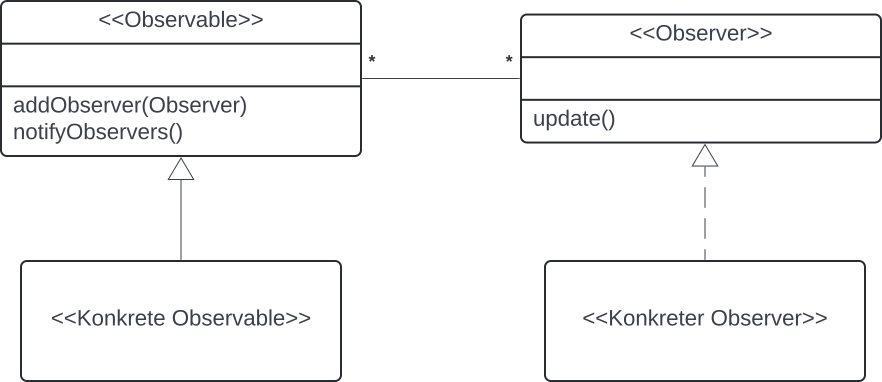
\includegraphics[scale=0.4]{part two/Objektorientierter Entwurf/img/observer}
        \caption{Klassendiagramm des Observer-Patterns (Quelle: eigene)}
        \label{fig:observer_cc}
    \end{figure}
    \begin{figure}
        \centering
        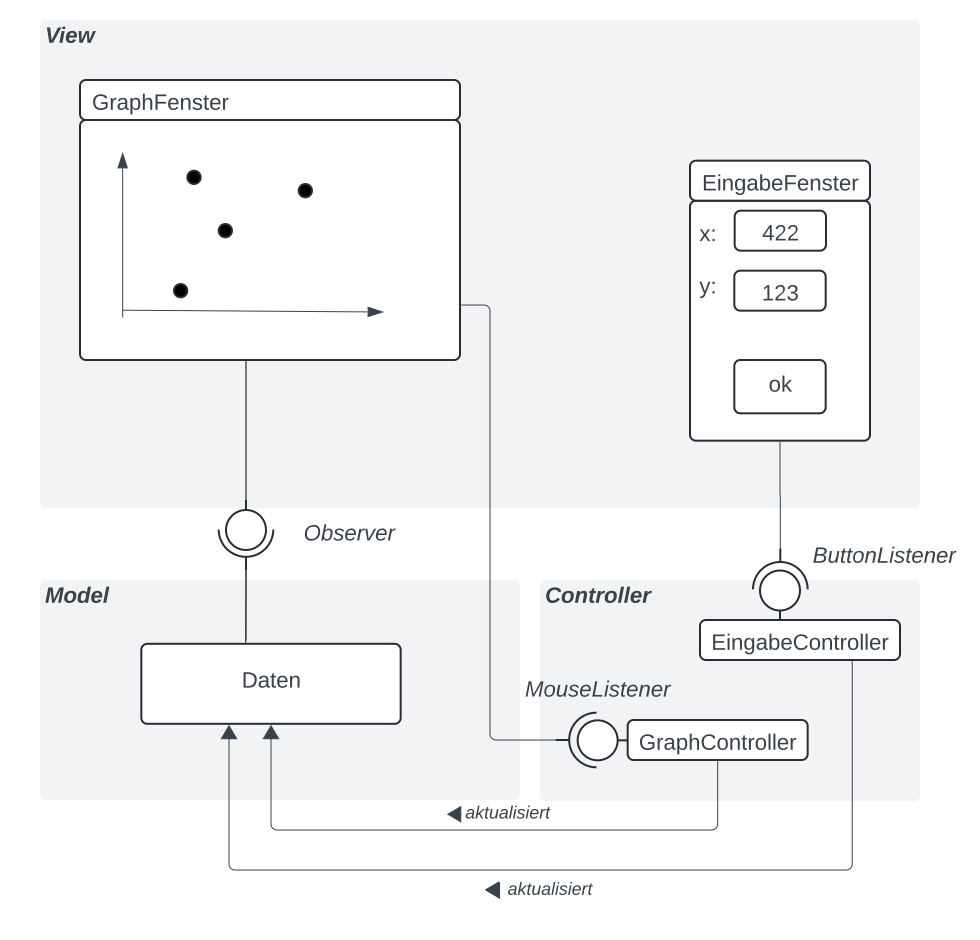
\includegraphics[scale=0.4]{part two/Objektorientierter Entwurf/img/mvc}
        \caption{Schematische Darstellung des MVC-Patterns mit seinen Verantwortlichkeiten (Quelle: eigene)}
        \label{fig:mvc_cc}
    \end{figure}
    \begin{figure}
        \centering
        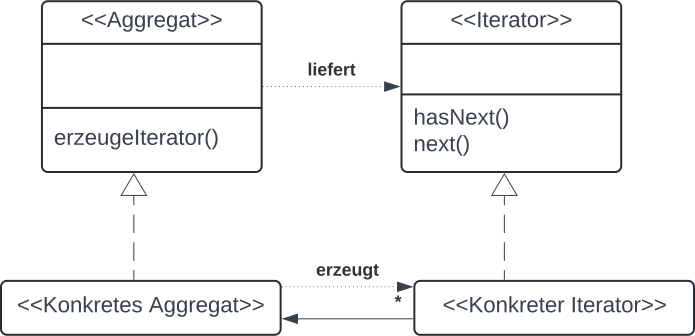
\includegraphics[scale=0.4]{part two/Objektorientierter Entwurf/img/iterator}
        \caption{Klassendiagramm des Iterator-Patterns (Quelle: in Anlehnung an~\cite[60, Abb. 3.9]{Wed09b})}
        \label{fig:iterator_cc}
    \end{figure}
\begin{figure}
    \centering
    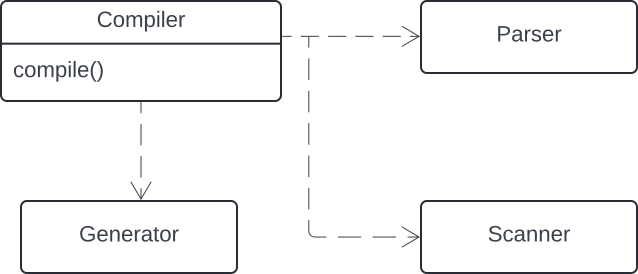
\includegraphics[scale=0.4]{part two/Objektorientierter Entwurf/img/fassade}
    \caption{Informelle Darstellung der Arbeitsweise einer Fassdade (Quelle: eigene)}
    \label{fig:fassade_cc}
\end{figure}

\clearpage


\section{Vorgehen beim Dialogentwurf}

\begin{tcolorbox}[title=Vorgehen beim Dialogentwurf]
    \begin{enumerate}
        \item Entscheiden, um welche prinzipielle Art der Anwendung es sich handelt
        \item \textbf{Informationsarchitektur} planen: Inhalte und Verteilung der Inhalte überlegen
        \item basierend auf diesen Überlegungen wird die äußere Struktur und das äußere Erscheinungsbild entworfen
    \end{enumerate}

    \noindent
    Grundlage für diese Arbeiten sind die \textbf{Anforderungen} und die bisherigen \textbf{Ergebnisse der Analyse}.
\end{tcolorbox}

\clearpage


\section{Vorgehen beim Entwerfen}

\begin{tcolorbox}[title=Vorgehen beim Entwerfen]
    \begin{enumerate}
        \item Aufteilung der User Story in Anwendungsfälle
        \item \textbf{Analyseergebnis}:
        \begin{itemize}
            \item  Aus den funktionalen Anforderungen extrahiert er das \textbf{Domänenmodell}, das in ein (wenig detailliertes) UML-Klassendiagramm überführt wird
            \item  ein \textbf{fachlicher Dialogentwurf} zeigt eine grobe Skizze des UI mit einigen Interaktionselementen
        \end{itemize}
        \item \textbf{Entwurf}:
        \begin{itemize}
            \item ein \textbf{technischer Dialogentwurf} erweitert den fachlichen Dialogentwurf um konkrete Typen der einzelnen Interaktionselemente und verwendeten Komponenten
            \item das Klassendiagramm der Analyse wird erweitert, Klassendiagramme der Komponenten werden hinzugefügt und um technischen Details ergänzt
        \end{itemize}
    \end{enumerate}
\end{tcolorbox}
\clearpage

\section{Prinzipien guten Entwurfs}

\begin{tcolorbox}[title=Prinzipien guten Entwurfs]

    \begin{itemize}
        \item \textbf{Generelle Prinzipien}
        \begin{itemize}
            \item Funktionsfähigkeit
            \item Änderbarkeit
        \end{itemize}
        \item \textbf{Grundlegende Prinzipien}
        \begin{itemize}
            \item Abstraktion:  das Herausheben von Wesentlichem;  ein Teil ist leichter zu verstehen, wenn nicht alle Details verstanden werden müssen, sondern nur das Wesentliche.
            \item Law of Demeter: ``Talk to friends, not to strangers.
            \item Vermeidung zirkulärer Abhängigkeiten
            \item Liskovsches Substitutionsprinzip: Objekte einer Klasse können durch andere Objekte davon abgeleiteter Klassen ersetzt werden; wenn ein bestimmter Typ gefordert ist, ist auch sein Untertyp erlaubt.
        \end{itemize}
        \item \textbf{Teile und Herrsche}
        \begin{itemize}
            \item Lösungen in Teillösungen aufteilen
            \item Systeme $\rightarrow$ Subsysteme $\rightarrow$ Pakete $\rightarrow$  Klassen $\rightarrow$ Methoden
        \end{itemize}
        \item \textbf{Hohe Kohäsion}
        \begin{itemize}
            \item Zusammenhang innerhalb der Teile hoch, Abhängigkeiten nach außen minimal
        \end{itemize}
        \item \textbf{Lose Kopplung}
        \begin{itemize}
            \item Kopplungen möglichst schwach halten, da die Teile der Software unabhängig voneinander sein sollen.
        \end{itemize}
    \end{itemize}

\end{tcolorbox}
\clearpage

\section{Typen des Zusammenhalts}


\begin{tcolorbox}[title=Typen des Zusammenhalts]

    Mit Absteigender Richtung wird der Zusammenhalt schwächer:

\begin{itemize}
    \item \textbf{Funktionaler Zusammenhalt}
    \begin{itemize}
        \item ähnliche Funktionalität wird in gleichen Softwareteilen implementiert
        \item die Funktionalität ist nach Möglichkeit nicht von anderer Funktionalität abhängig und besitzt keine Nebeneffekte
        \item Idealfall: Eine Operation liefert ein bestimmtes Ergebnis und ist unabhängig von vorausgegangen Aufrufen, internen Zuständen oder Teilen des Systems
        \item Forderung nach Unabhängigkeit allerdings meist nicht möglich, da in der Objetorientierung Objekte i.d.R. über Attribute interne Zustände besitzen (s. Abbildung~\ref{fig:adt}); außerdem benutzen Klassen anderen Klassen, oder externe Systeme wie Datenbanken
    \end{itemize}

    \item \textbf{Schichten-Zusammenhalt}
    \begin{itemize}
        \item Teile, die ähnliche Services für andere Teile zur Verfügung stellen, werden in Schichten zusammengefügt (s. Abschnitt~\ref{sec:architekturmuster})
    \end{itemize}
    \item \textbf{kommunikativer Zusammenhalt}
    \begin{itemize}
        \item Teile, die auf gleichen Daten operieren, gehören zusammen
        \item der Zusammenhalt ist an der Stelle schwächer als der Schichten-Zusammenhalt, da man i.d.R. nicht Geschäftslogik und Zugriff auf Datenbanken in derselben Klasse implementiert, auch, wenn das Model dieselben Daten benötigt
    \end{itemize}
    \item \textbf{Utility-Zusammenhalt}
    \begin{itemize}
        \item unter ``\textit{Utility}`` werden hier Teile gemeint, die ähnliche Funktionalität bereitstellen, sich aber logisch nicht ordnen lassen (bspw. in Schichten)\footnote{s. bspw. Klassen aus \url{https://docs.oracle.com/en/java/javase/21/docs/api/java.base/java/util/package-summary.html}, abgerufen 19.04.2024}
    \end{itemize}
\end{itemize}
    \end{tcolorbox}
\clearpage

\section{Typen der Kopplung}


\begin{tcolorbox}[title=Typen der Kopplung]
    \begin{itemize}
        \item \textbf{Content-Kopplung}
        \begin{itemize}
            \item ein Teil ändert interne Daten eines anderen Teils
            \item die ändernde Klasse ist von der Struktur der zu ändernden Klasse \textbf{abhängig}
        \end{itemize}
        \item \textbf{Common-Kopplung}
        \begin{itemize}
            \item bezeichnet Kopplung über die gemeinsame Verwendung globaler Variablen
        \end{itemize}
        \item \textbf{Stamp-Kopplung}
        \begin{itemize}
            \item ein Objekt wird als Argument einer Methode verwendet
            \item wird der öffentliche Teil der Klasse des Objektes geändert, muss auch die aufrufende Methode geändert werden
        \end{itemize}
        \item \textbf{Data-Kopplung}
        \begin{itemize}
            \item je mehr Argumente eine Methode hat, desto größer ist die Kopplung mit der benutzenden Komponente
        \end{itemize}
        \item \textbf{Routine Call-Kopplung}
        \begin{itemize}
            \item eine Methode ruft eine andere Methode auf
            \item werden sehr viele Methode eines anderen Teils aufgerufen, sollte man die Zerlegung überlegen
            \item werden Methoden immer in gleicher Sequenz aufgerufen, könnte man überlegen, die Sequenz auch als eigenständige Methode zusammenfassen
        \end{itemize}
    \end{itemize}
\end{tcolorbox}

\clearpage

\section{Refactoring}

\begin{tcolorbox}[title=Refactoring]
Unter \textbf{Refactoring} bezeichnet man die systematische Verbesserung des Entwurfs von Software, ohne dabei die Funktionalität zu ändern.
\end{tcolorbox}
\clearpage